\documentclass{beamer}
%Information to be included in the title page:

\usepackage{svg}

\title{Concurrent Map Reduce (CMR)}
\author{Guillaume Dindart \\[1ex] \small Gilles MARAIT (Encadrant), Emmanuel AGULLO (Encadrant) \\ Équipe Concace INRIA}
\date{2024}

\begin{document}

\frame{\titlepage}


\begin{frame}
    \frametitle{Dot product}
    \begin{columns}[T]
        \begin{column}{0.5\textwidth}  %%<--- here
            \begin{minipage}[t][.5\textheight]{\textwidth}
                \begin{center}
                    \includesvg[height=0.4\textheight]{figures/dot_product.drawio.svg}
                \end{center}
            \end{minipage}\par
            \begin{minipage}[t][.5\textheight]{\textwidth}
                \begin{equation*}
                    \begin{split}
                        \alpha = x_1 \times y_1  \\
                        \alpha += x_2 \times y_2 \\
                        \alpha += x_3 \times y_3 \\
                        \alpha += x_4 \times y_4
                    \end{split}
                \end{equation*}
            \end{minipage}
        \end{column}

        \begin{column}{0.5\textwidth}
            \begin{minipage}[t][.5\textheight]{\textwidth}
                \begin{center}
                    \includesvg[height=0.5\textheight]{figures/dag_STF.drawio.svg}
                \end{center}
            \end{minipage}\par
            \begin{minipage}[t][.5\textheight]{\textwidth}
                Using reduce to optimize?
            \end{minipage}


        \end{column}
    \end{columns}
\end{frame}


\begin{frame}
    \frametitle{Sequential Task Flow (STF)}
    \begin{columns}[T]
        \begin{column}{0.5\textwidth}  %%<--- here
            \begin{minipage}[t][.5\textheight]{\textwidth}
                \begin{center}
                    \includesvg[height=0.4\textheight]{figures/dot_product.drawio.svg}
                \end{center}
            \end{minipage}\par
            \begin{minipage}[t][.5\textheight]{\textwidth}
                \begin{equation*}
                    \begin{split}
                        \alpha_1 = x_1 \times y_1  \\
                        \alpha_2 = x_2 \times y_2 \\
                        \alpha_3 = x_3 \times y_3 \\
                        \alpha_4 = x_4 \times y_4 \\ 
                        Reduce(\alpha_1,\alpha_2,\alpha_3,\alpha_4)
                    \end{split}
                \end{equation*}
            \end{minipage}
        \end{column}

        \begin{column}{0.5\textwidth}
            \begin{minipage}[t][.5\textheight]{\textwidth}
                \begin{center}
                    \includesvg[height=0.2\textheight]{figures/dag_mr.drawio.svg}
                \end{center}
            \end{minipage}\par
            \begin{minipage}[t][.5\textheight]{\textwidth}
                Advantage:
                \begin{itemize}
                    \item Natural to pipeline
                \end{itemize}
                Disadvantage:
                \begin{itemize}
                    \item Dynamic control flow
                \end{itemize}
                Question:
                \begin{itemize}
                    \item Similar stencil ?
                \end{itemize}
            \end{minipage}


        \end{column}
    \end{columns}
\end{frame}

\begin{frame}
    \frametitle{Map Reduce (MR)}
    \begin{columns}[T]
        \begin{column}{0.5\textwidth}  %%<--- here
            \begin{minipage}[t][.5\textheight]{\textwidth}
                \begin{center}
                    \includesvg[height=0.4\textheight]{figures/dot_product.drawio.svg}
                \end{center}
            \end{minipage}\par
            \begin{minipage}[t][.5\textheight]{\textwidth}
                Map = $\times$ and Reduce = +
                \begin{equation*}
                    \begin{split}
                        \alpha _1 = Map(x_1, y_1) \\
                        \alpha _2 = Map(x_2, y_2) \\
                        \alpha _3 = Map(x_3, y_3) \\
                        \alpha _4 = Map(x_4, y_4) \\
                        \alpha = Reduce(\alpha _1, \alpha _2, \alpha _3, \alpha _4)
                    \end{split}
                \end{equation*}
            \end{minipage}
        \end{column}
        \begin{column}{0.5\textwidth}
            \begin{minipage}[t][.5\textheight]{\textwidth}
                \begin{center}
                    \includesvg[height=0.2\textheight]{figures/dag_mr.drawio.svg}
                \end{center}
            \end{minipage}\par
            \begin{minipage}[t][.5\textheight]{\textwidth}
                Advantage:
                \begin{itemize}
                    \item Static control flow
                \end{itemize}
                Question :
                \begin{itemize}
                    \item How to make a matrix product with it?
                \end{itemize}
            \end{minipage}
        \end{column}
    \end{columns}
\end{frame}

\begin{frame}
    \frametitle{Concurrent Map Reduce (CMR): Matrix product (GEMM)}

    \begin{columns}[T]
        \begin{column}{0.5\textwidth}  %%<--- here
            \begin{minipage}[t][.5\textheight]{\textwidth}
                \begin{center}
                    \includesvg[height=0.4\textheight]{figures/matrix_product.drawio.svg}
                \end{center}
            \end{minipage}\par
            \begin{minipage}[t][.5\textheight]{\textwidth}
                Each coordinate in C correspond in one MapReduce operation.
                \newline

                Concurrent Map Reduce = multiple simultaneous Map Reduce
            \end{minipage}
        \end{column}
        \begin{column}{0.5\textwidth}
            \begin{minipage}[t][.5\textheight]{\textwidth}
                    Datamap: Who has what block
                    
                    Taskmap: Who works on which block
            \end{minipage}\par
            \begin{minipage}[t][.5\textheight]{\textwidth}
                How to pipeline multiple CMR?
            \end{minipage}
        \end{column}
    \end{columns}
\end{frame}

\begin{frame}
    \frametitle{CMR: Pipeline (D = $(A \times B) \times C$)}
    \begin{columns}[T]
        \begin{column}{0.5\textwidth}  %%<--- here

            \begin{center}
                \includesvg[height=0.8\textheight]{figures/matrix_3_product.drawio.svg}
            \end{center}

        \end{column}
        \begin{column}{0.5\textwidth}
            Tasks submission
            \begin{minipage}[t][.2\textheight]{\textwidth}
                With datamap and taskmap, we generate all the tasks. When a block is calculated, we send it to the other nodes if they need it.
            \end{minipage} \par
            \begin{minipage}[t][.33\textheight]{\textwidth}
                Without pipeline
                \begin{center}
                    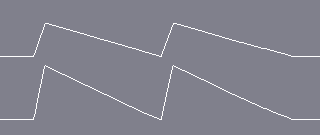
\includegraphics[width=0.8\textwidth]{figures/no-pipeline_submit.png}
                \end{center}
            \end{minipage}\par
            \begin{minipage}[t][.33\textheight]{\textwidth}
                With pipeline
                \begin{center}
                    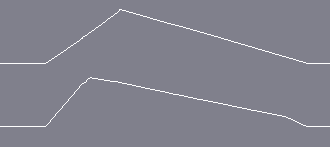
\includegraphics[width=0.8\textwidth]{figures/pipeline_submit.png}
                \end{center}
            \end{minipage}
        \end{column}
    \end{columns}
\end{frame}

\begin{frame}
    \frametitle{CMR: Pipeline CPU sleeping}

    \begin{minipage}[t][.5\textheight]{\textwidth}
        Without pipeline
        \begin{center}
            \includesvg[inkscapelatex=false, width=0.8\textwidth]{figures/CMR/no-pipeline.svg}
        \end{center}
    \end{minipage}\par
    \begin{minipage}[t][.5\textheight]{\textwidth}
        With pipeline
        \begin{center}
            \includesvg[inkscapelatex=false, width=0.8\textwidth]{figures/CMR/pipeline.svg}
        \end{center}
    \end{minipage}

\end{frame}

\begin{frame}
    \frametitle{On going}
    \begin{itemize}
        \item More general CMR:
              \begin{itemize}
                  \item OpenMP backend instead of StarPU
                  \item TRSM algorithm (Hugo pre-thesis)
              \end{itemize}
        \item Vectorization of Map and Reduce (presentation by Aurélien)
    \end{itemize}

\end{frame}

\end{document}